\chapter{Literature surveys}
As stated, this project involves the combination of multiple components, each of which has an extensive research scene behind them. A thorough understanding of  these components, obtained through reviewing research literature, is crucial for implementing them into our project correctly. 

\section{Wake-Up-Word Spotting for Mobile Systems\cite{wuwmobile}}
Our trigger word detection follows the method described in this paper . The paper proposes a system to spot wake-up words in continuous audio for use on a mobile system. The key constraints listed are:  speaker dependent spotting, use of individual personalized keyword, no transcription of the keyword, no training phase, low power and computing resources, and in general a language-independent system. The system is implemented using template-matching  with DTW. Other algorithms such as Euclidian Distance and Cross Correlation are used alongside DTW to increase accuracy.

The aim of the research is to achieve a precision of more than 95\% at an acceptable recall of more than 50\%. This means that about half of the WUW are detected correctly while almost all triggered detection are correct. As the goal is to prioritize precision over recall, motivated by the need to  not triggering too many false alarms, the best combination of the distance measures is determined by weighting the precision three times more important than the recall. Testing in different environments with low, medium and high level of noise yields an average precision of 99.7\% and recall of 56.9\%.
\begin{figure}[h]
    \centering
    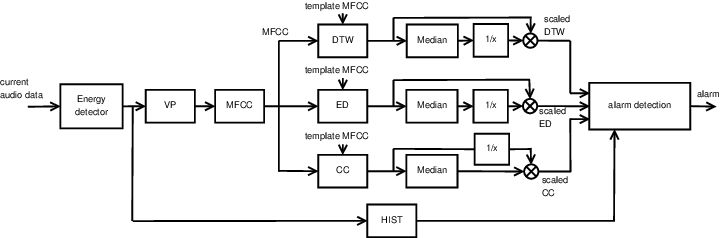
\includegraphics[width = 0.9\textwidth]{img/WUW-spotting-system.png}
    \caption{WUW spotting system}
    \label{fig:lr1l}
\end{figure}
\section{Keyword Spotting based on the Analysis of Template Matching Distances\cite{barakat}}
This literature covers a Keyword Spotting(KWS) system to spot certain keywords in continuous speech using spoken example templates. The approach proposed also use DTW for pattern matching, requiring no modelling or training. This article briefly pointed out some limitations of DTW based matching with fixed threshold, alongside other methods for KWS such as Hidden Markov Model (HMM) and phone/word recognizer. When operating with a fixed threshold, DTW models typically suffer problems regarding the computational complexity, determining the appropriate similarity threshold\cite{wilpon} and the poor modeling of word duration.\cite{yadong}

To address this problem, the article introduced the use of the DTW distance histogram for automatic estimation of similarity thresholds for every keyword-utterance pair.This proposed approach depends on a hypothesis that the distance between the word template and sections of the utterance containing the word is small compared with the distance resulting from comparisons of the template with other parts of the utterance that do not contain the word. This should apply regardless of speakers and dialects.The proposed KWS is designed based on this hypothesis; the template is compared with varying length segments,centered at each analysis frame of the utterance, and the resulting minimum distance and corresponding frame number are recorded. 

The entire process is described through the figure included. The result from experiments on various keywords varies, with some giving very high or low recall/precision. The system can achieve a recall higher than 73\% but with low precision. The top two most reasonable setup resulted in 57.5\%, 55\% recall and 44.8\%, 47.6\% precision respectively.
\begin{figure}[h]
    \centering
    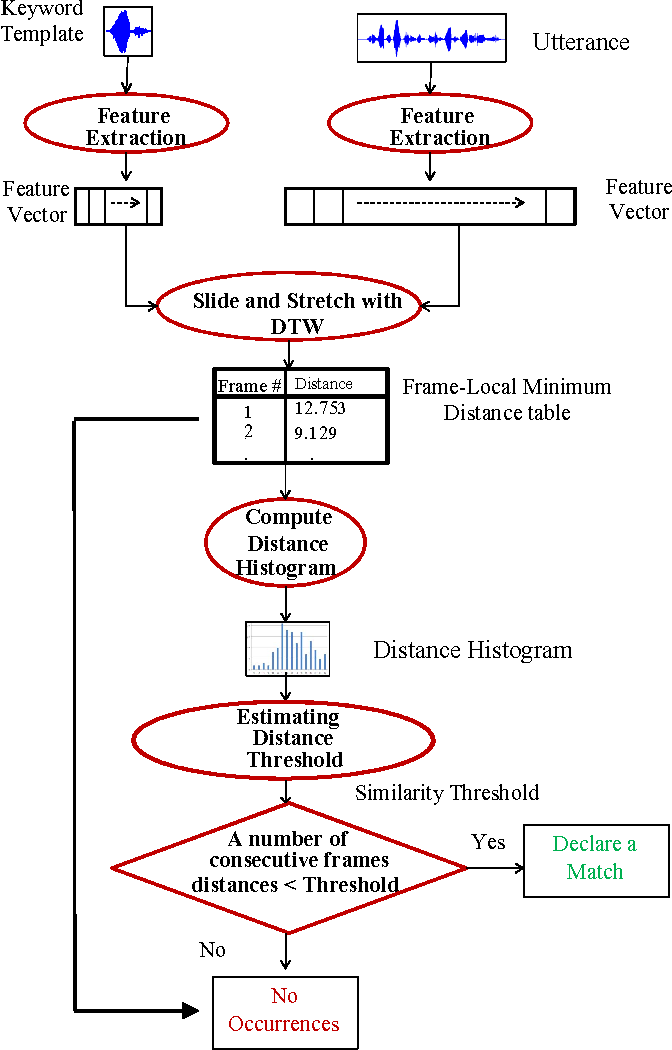
\includegraphics[height=15cm]{img/kws_lr2.png}
    \caption{The proposed KWS system}
    \label{fig:lr2}
\end{figure}
